\documentclass{article}

% if you need to pass options to natbib, use, e.g.:
%     \PassOptionsToPackage{numbers, compress}{natbib}
% before loading neurips_2020



% to compile a preprint version, e.g., for submission to arXiv, add add the
% [preprint] option:
%     \usepackage[preprint]{neurips_2020}

% to compile a camera-ready version, add the [final] option, e.g.:
\usepackage[final]{neurips_2020}

% to avoid loading the natbib package, add option nonatbib:
     %\usepackage[nonatbib]{neurips_2020}

\usepackage[utf8]{inputenc} % allow utf-8 input
\usepackage[T1]{fontenc}    % use 8-bit T1 fonts
\usepackage{hyperref}       % hyperlinks
\usepackage{url}            % simple URL typesetting
\usepackage{booktabs}       % professional-quality tables
\usepackage{amsfonts}       % blackboard math symbols
\usepackage{nicefrac}       % compact symbols for 1/2, etc.
\usepackage{microtype}      % microtypography

% Our packages
\usepackage{graphicx}       % images
\usepackage{float}          % images
\usepackage{amsmath}        % math

\title{Advanced Machine Learning, Fall 2023}

% The \author macro works with any number of authors. There are two commands
% used to separate the names and addresses of multiple authors: \And and \AND.
%
% Using \And between authors leaves it to LaTeX to determine where to break the
% lines. Using \AND forces a line break at that point. So, if LaTeX puts 3 of 4
% authors names on the first line, and the last on the second line, try using
% \AND instead of \And before the third author name.

\author{%
  Thomas Kientz \\
  ENSAE Paris\\
  \texttt{thomas.kientz@ensae.fr} \\
  \And
  Elena Loumagne \\
  ENSAE Paris\\
  \texttt{elena.loumagne@ensae.fr} \\
  \AND
  Adèle Moreau \\
  ENSAE Paris\\
  \texttt{adele.moreau@ensae.fr} \\
}

\begin{document}

\maketitle

\begin{abstract}
  This study focuses on removing the background from datasets of faces to gauge the effect on the training and performance of facial generative models. We are also interested on the effect on the interpretability of the latent spaces of the models. 
\end{abstract}

\section{Introduction}

\quad The realm of image generation has seen some major breakthroughs in recent years. 
An area of specific interest to us was that of the latent representations of complex images in generative models. 
Observing these gives us an insight into what best characterizes an image, in the eyes of the trained algorithm. 
When applied to a dataset of human faces, they can give us objective* (*depending on dataset bias…) insight into our most defining traits.

Most image generation techniques will create an image from a scalar vector as input. 
During training, the algorithm will learn to map the dimensions of input vectors to different aspects of the image. 
This vector is what we are calling the latent vector, and its shape is the latent dimension. 
It can very well be interpreted as a compressed version of the image - indeed, a 128x128x3 RGB image is 49k+ scalars, and latent dimension is typically chosen to have 64-512 scalars. 

The key observation that we made was that in many trained face generation algorithms, the background of the image occupied a large portion* (* metrics discussed later - PCA eigenvalues) of the captured variance - i.e. of the latent space. 
This means that some precious space from the latent vector is wasted on encoding what is behind the face, instead of the face itself. 

There are a few neutral-background datasets, but none of them have nearly enough samples to train generative algorithms, and are mostly used to train or fine tune classifiers (https://libguides.princeton.edu/facedatabases). 
We should aim for 10k-100k+ unique images, but none here exceed 1k with a neutral background.

\section{Related work}

\quad For the face generation task, some authors decided to circumvent the effect of the background by using a cropped version of their dataset to prevent various noisy backgrounds (Gauthier, 2014) from interacting with the model. 
Jon Gauthier. 2014. Conditional Generative Adversarial Nets for Convolutional Face Generation. Technical Report. Stanford University (https://www.foldl.me/uploads/2015/conditional-gans-face-generation/paper.pdf)

In a context of face generation with emotions with Sinha et al, 2022, the background issue is also circumvented by first replacing the background of the original image with a specific color  (solid dark green) and, as post-processing, the background of the original image is then added back to the generated image. 
The goal of the authors was different though - they only did this because the “emotions” dataset they used to train their model (MEAD) had a solid dark green background.

Sanjana Sinha, Sandika Biswas, Ravindra Yadav, and Brojeshwar Bhowmick. Emotion-controllable generalized talking face generation. International Joint Conferences on Artificial Intelligence Organization, 2022. (https://arxiv.org/pdf/2205.01155.pdf)

The impact of the background removal on Convolutional Neural Networks has been proved for classification tasks (KC and al., 2021). Achieving a 12\% higher accuracy on the task of Plant Disease Classification In-Situ for a dataset with images taken with a homogeneous background compared to that of a dataset with a cluttered background.
KC, K.; Yin, Z.; Li, D.; Wu, Z. Impacts of Background Removal on Convolutional Neural Networks for Plant Disease Classification In-Situ. Agriculture 2021, 11, 827. (https://www.mdpi.com/2077-0472/11/9/827)

All these tricks suggest an important effect of the background on image generation. 
However, we have not found any studies on the importance of this effect of the background on image generation, and particularly face generation.

\section{Methodology}

\quad Our idea was to create our own neutral-background dataset, from a normal face dataset, the Flicker-Faces-HQ dataset, often used for facial generation tasks. 

To do this, we first decomposed the image by isolating the face and background using the \texttt{rembg} library. 
Then we created two datasets, one with a large Gaussian blur background and the other with a grey background. 
With over 70,000 images, our neutral background datasets are effective for training generative algorithms.

We focused on the 128x128 resolution version of the FFHQ dataset.
The datasets we generated were uploaded to Kaggle \hyperlink{https://www.kaggle.com/thomaskientz/datasets}{on this link}.

\textbf{Our main hypothesis is that the removal of the background will have a positive impact on the performance and the training of the generative models. 
Furthermore, we expect the latent space to be more interpretable.}

\begin{figure}[H]
    \centering
    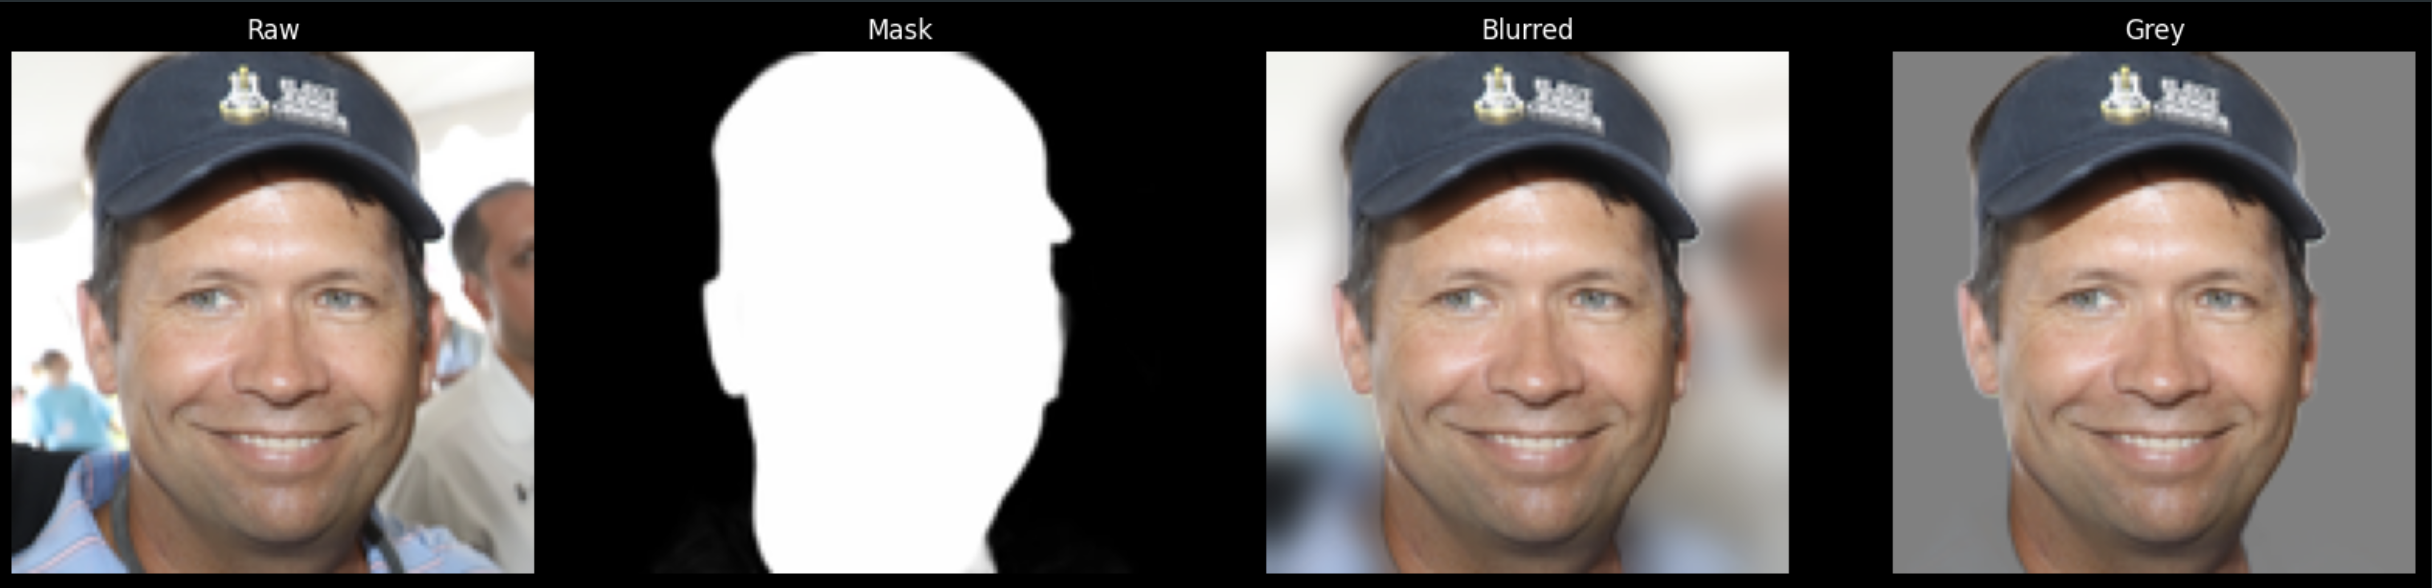
\includegraphics[width=0.8\textwidth]{images/mask.png}
    \caption{From left to right, original image, mask, blurred, greyed-out}
\end{figure}

To test our hypothesis, we trained models on both the original and the greyed-out versions of the same dataset. 
We picked versions of the two main categories of generative models: Autoencoders (AE) and Generative Adversarial Networks (GAN).

\subsection{Auto-encoders}
\subsubsection*{Principle - Auto-encoders}

\quad Autoencoders are unsupervised artificial neural networks whose main objective is to learn efficient representations of input data. 
An autoencoder consists of two sub-networks: an encoder and a decoder. 
Firstly, the encoder compresses the input data (image) into a lower-dimensional representation. 
It reduces the dimensionality of the input data by mapping it to a set of hidden variables, often referred to as 'latent space'. 
The decoder then takes the encoded representation and reconstructs the original input data from it. 
The aim is to minimize the difference between the input and the reconstructed output, encouraging the model to learn a meaningful and compact representation.

\begin{figure}[H]
    \centering
    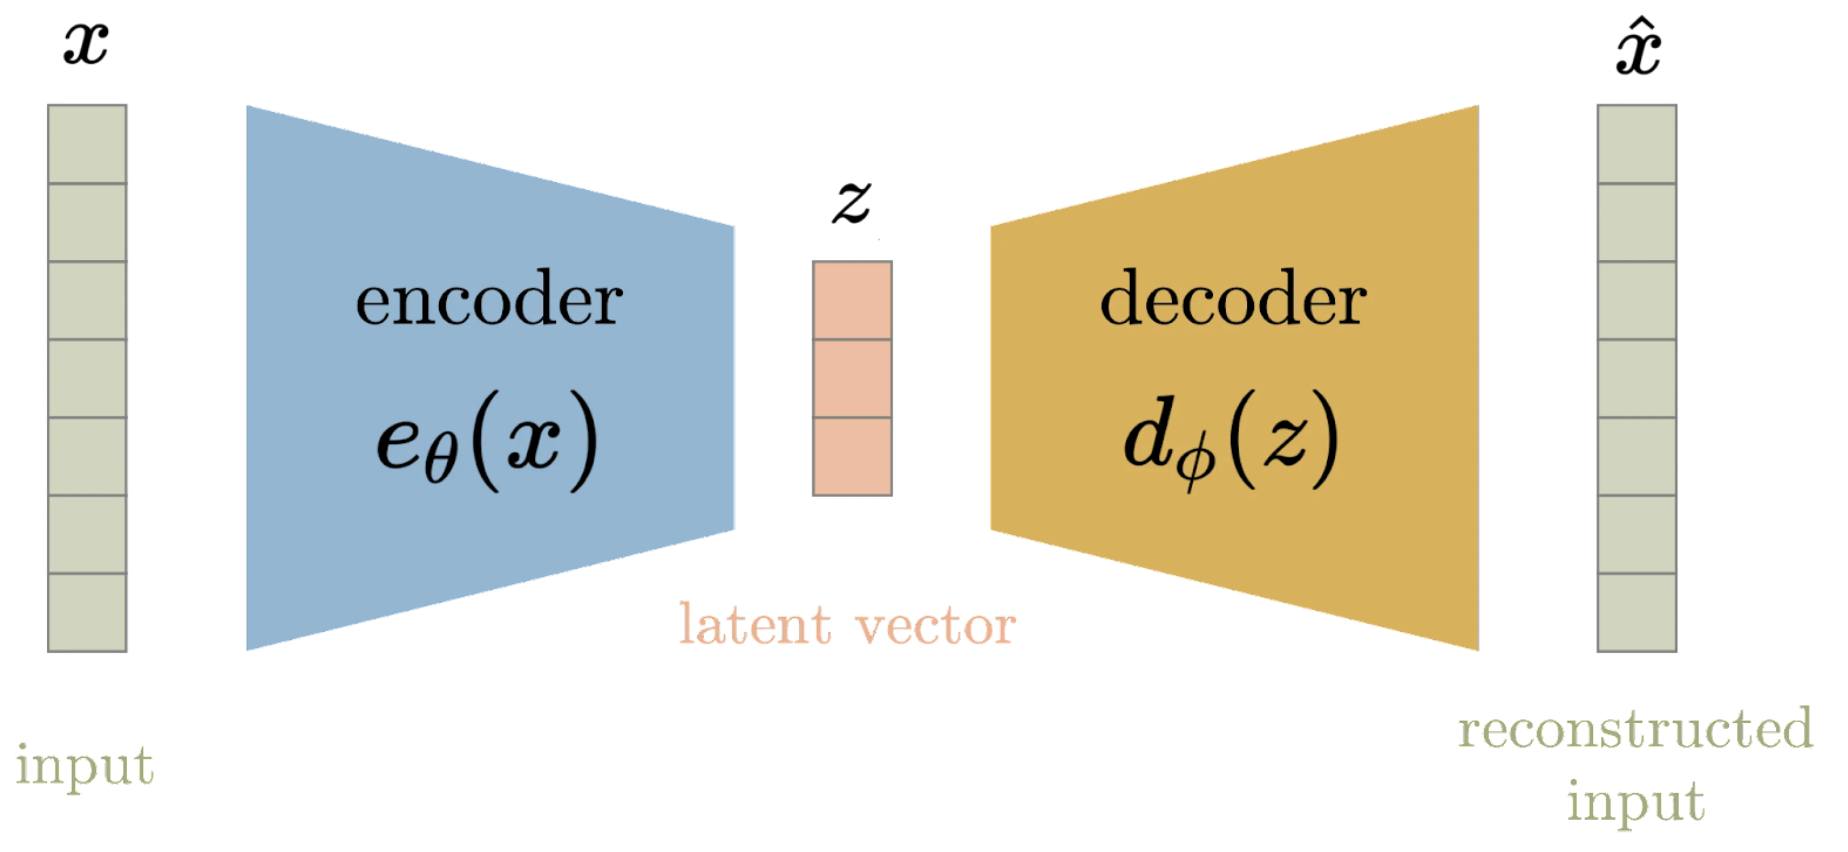
\includegraphics[width=0.6\textwidth]{images/ae.png}
    \caption{Autoencoder architecture}
\end{figure}

Let $e_{\theta}:\mathcal{X}\to \mathcal{F}$ be the encoder function and $d_{\phi}:\mathcal{F}\to \mathcal{X}$ the decoder function. 
During training, input image $x$ is fed to the encoder function and passed through a series of layers that reduce their dimensions to give a compressed latent vector $z$. 
The number, type and size of the layers, as well as the size of the latent space, are parameters that can be controlled. 
Next, the decoder function maps the $\mathcal{F}$ latent space at the bottleneck to the output, attempting to recreate the original image after some generalized non-linear compression. 

The loss function used to train the neural network through the backpropagation procedure is as follows: 

\[\mathcal{L}(x,\hat{x})=\left\| x-\hat{x}\right\|_{2}=\left\| x-d_{\phi}(e_{\theta}(x)) \right\|_{2}\]

There is a trade-off between quality and latent dimensionality. Below a certain point, the latent space is too small to capture the important features of the input data, and all the images look the same.
This means that latent space of an autoencoder also subject to irregularity due to overfitting. 

\subsubsection*{Principle - Variational Auto-encoders}
To tackle this problem, King et al. in 2013 proposed the Variational Autoencoder (VAE) architecture. It addresses the problem of irregular latent space in a conventional autoencoder by mapping inputs to parameters of a probability distribution instead of a fixed vector.
The VAE then imposes a constraint on this latent distribution, forcing it to be a Gaussian distribution, ensuring that the latent space is regularized.

\begin{figure}[H]
    \centering
    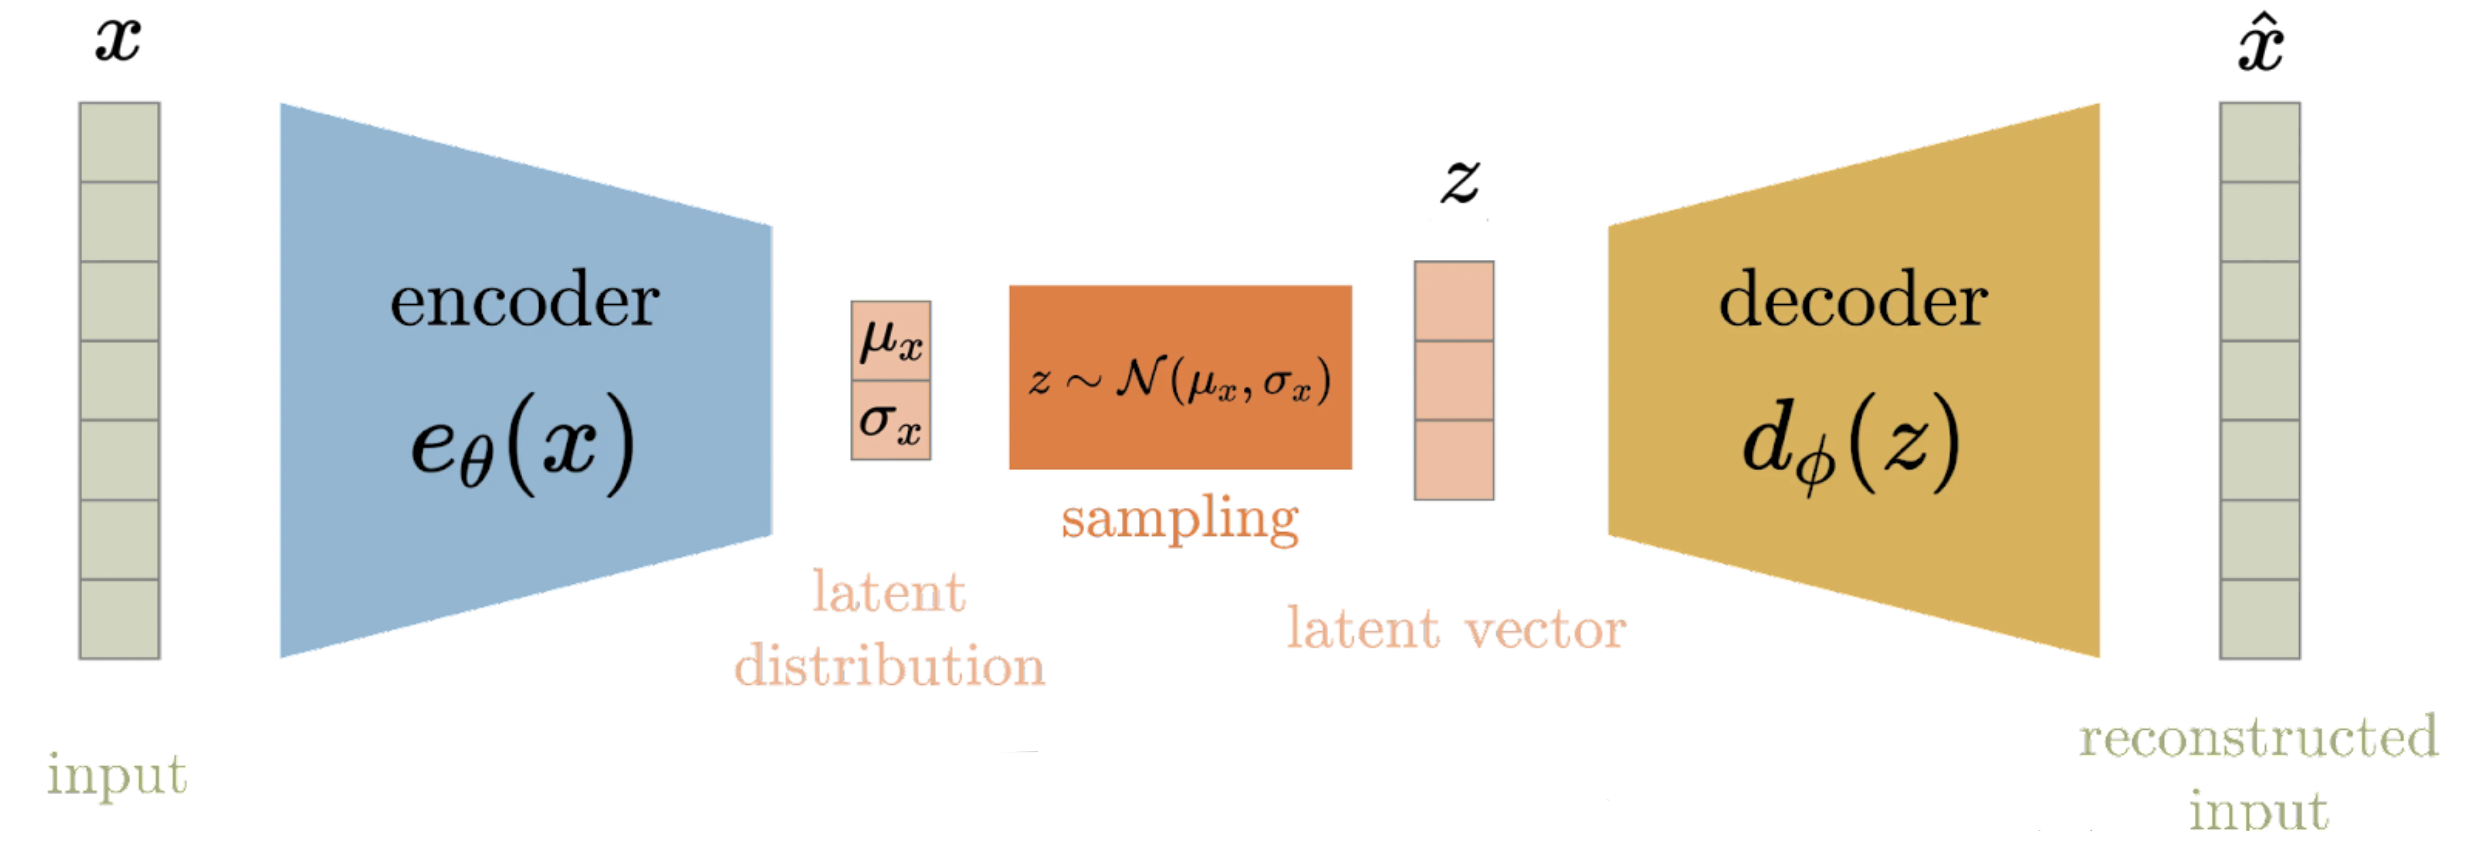
\includegraphics[width=0.8\textwidth]{images/vae.png}
    \caption{Variational Autoencoder architecture}
\end{figure}

The VAE's encoder outputs the mean and standard deviation for each latent variable. The latent for the decoder is sampled from that distribution.
The VAE loss function takes into account two terms, the reconstruction loss and the similarity loss (regularizer). 
The regularizer corresponds to the Kullback-Leibler divergence between the latent space distribution and a standard Gaussian distribution.
  
We can define the reconstruction loss as follows:
$$\text{reconstruction loss} = \left\| x -\hat{x}\right\|_{2}=\left\| x-d_{\phi}(z) \right\|_{2}=\left\| x-d_{\phi}(\mu_{x}+\sigma_{x}\epsilon) \right\|_{2}$$

where
$$\mu_{x},\sigma_{x}=e_{\theta(x)} \text{ and } \epsilon\sim\mathcal{N}(\textbf{0},\textbf{I})$$


And the similarity loss:
$$\text{similarity loss}=\mathrm{D}_{\mathrm{KL}}(\mathcal{N}(\mu_{x},\sigma_{x}), \mathcal{N}(\textbf{0},\textbf{I})) \\$$

Finally,
$$\text{loss}=\text{reconstruction loss}+\text{similarity loss}$$

\subsubsection*{Rationale for choosing VAE}
VAEs generally perform better than regular AEs in image generation tasks. 
First, by learning a probabilistic latent space representation, it allows for smoother transitions and better interpolation in the latent space, which is crucial for generating diverse and realistic images. 
Then, VAEs inherently include a regularization term in their objective function, which encourages the learned latent space to be well-structured. 
This regularization helps prevent overfitting and aids in disentangling meaningful features in the latent space.
  
This is especially important for us, since we want to be able to interpret the latent space of our models.


\subsection{Generative Adversarial Networks}
\subsubsection*{Principle - Generative Adversarial Networks}
\quad Introduced by Ian Goodfellow and al. in 2014, the Generative Adversarial Network consists of a Generator and a Discriminator, two neural networks that are trained simultaneously by adversarial training. \\
Firstly, the Generator model attempts to model the distribution of data in order to generate realistic samples. 
It takes as input a random noise sample of fixed size from a latent space and generates new false images. 
The main objective is to fool the Discriminator by transforming the random noise into images indistinguishable from the real ones, making it harder to classify images as true or false. 
Then, acting like a binary classifier, the Discriminator attempts to classify the input data as real or generated one. \\

The generator and discriminator are trained in a loop, with the generator trying to improve its ability to generate realistic samples and the discriminator improving its ability to distinguish between real and fake samples. 
A loss is then measured and back propagated to update the weights of the two models. 
Training stops when the generated images look like real images.\\
In other words, the Generator and the Discriminator play the following two-player minimax game :
$$ \min_G \max_D V(D, G) = \mathbb{E}_{\mathbf{x} \sim p_{\text{data}}(\mathbf{x})} [\log D(\mathbf{x})] + \mathbb{E}_{\mathbf{z} \sim p_{\text{latent}}(\mathbf{z})} [\log (1 - D(G(\mathbf{z})))] $$

where:

\begin{itemize}
    \item $\mathbf{z}$ is a random noise vector drawn from the latent space distribution 
    \item $D(\mathbf{x})$ is the output of the discriminator for a real data sample
    \item $D(G(\mathbf{z}))$ is the output of the discriminator for a generated data sample
\end{itemize}

The discriminator tries to maximize the objective function while the generator tries to minimize the objective function. This is what we call adversarial training where the loss of one is the benefit of the other. By alternating between gradient ascent and descent, the network can be trained.\\

According to the authors of the article, in practice, the Generator objective function does not provide sufficient gradient to allow good learning. At the start of the training, when the sample is likely to be classified as false by the Discriminator, the function $\log(1 - D(G(z)))$  saturates because the gradients are relatively flat. As a result, the Generator is trained to maximize $log(D(G(z)))$, which provides much stronger gradients early in the learning. Thus, Instead of minimizing the likelihood of the Discriminator being correct, we maximize the likelihood of the Discriminator being wrong. 

\subsubsection*{Principle - Deep Convolutiobnal Generative Adversarial Networks}
In practice, “vanilla” GANs are hard to train and do not yield very realistic results, by 2024 standards. The first improvement we implemented over the standard GAN architecture was to use deep convolutions (and deconvolutions) for the Generator (and Discriminator), making it a DC-GAN (Deep Convolutional GAN). When dealing with image data, convolutions are more spatially aware than regular fully-connected layers because they only “mix” the values of pixels close together.

While more efficient than plain GANs, DCGANs have not been shown to generate realistic images. Their latent space is also very disorganized and hard to interpret. To tackle both of these problems, we decided to implement a custom version of NVidia’s StyleGAN, from scratch. StyleGANs are a variety of Progressive Growing GANs, which we will discuss in the next section.

\subsubsection*{Principle - ProGANs}
One of the key features of the ProGAN architecture is the progressive nature of the layers, which enables the different visual characteristics of an image to be taken into account effectively. 
The concept is simple: the lower the layer and resolution, the greater the impact on coarser features. 
This granularity means that the inputs at each level can be modified independently, allowing precise control of the visual elements, from general characteristics to complex details, without affecting the other levels. 
The result is the generation of high-resolution images with a higher level of authenticity than previous models.


\begin{figure}[H]
    \centering
    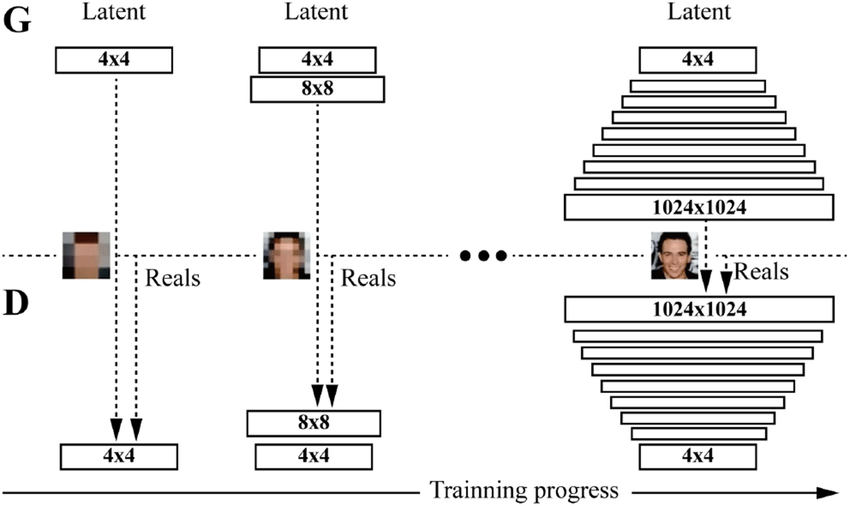
\includegraphics[width=0.8\textwidth]{images/progan.png}
    \caption{ProGAN training}
\end{figure}

In practice, the generator and discriminator are initialized with the full number of levels, but not all are used at first. Let's see the generation of an image at level 0 (i.e. at resolution 4x4):

\[\text{image}_{4x4}(z) = \text{ToRGB}_{4x4}(G_{4x4}(z))\]
\[\text{critic}_{4x4}(\text{image}) = D_{4x4}(\text{FromRGB}_{4x4}(\text{image}))\]

Now, at level 1 (resolution 8x8):

\[\text{image}_{8x8}(z) = \text{ToRGB}_{8x8}(G_{8x8}(G_{4x4}(z)))\]
\[\text{critic}_{8x8}(\text{image}) = D_{4x4}(D_{8x8}(\text{FromRGB}_{8x8}(\text{image})))\]

To prevent an explosion of gradients during the transition, we introduce $\alpha \in \left[0, 1\right]$, a parameter that controls the degree of blending between the two levels.

\[\text{image}_{8x8}(z, \alpha) = \alpha \times \text{image}_{8x8}(z) + (1-\alpha) \times Upscale(\text{image}_{4x4}(z))\]
\[\text{critic}_{8x8}(\text{image}, \alpha) = \alpha \times \text{critic}_{8x8}(\text{image}) + (1-\alpha) \times \text{critic}_{4x4}(DownScale(\text{image}))\]

The $\alpha$ parameter is increased linearly from 0 to 1 during the transition between levels 0 and 1. This process is repeated until the highest level is reached. 

ProGAN yields much better results than conventional GANs, but the latent space is still very disorganized and hard to interpret.

\subsubsection*{Principle - StyleGAN}

The main contribution of StyleGAN is in introduce a style-vector $w$ in the generator.

In each forward pass, a Mapping network $\mathcal{M}$ is used to map the latent vector $z$ to the intermediate latent space of styles, $w$.
Then, the generator $G$ uses $w$, instead of $z$, to generate the image. It also uses a learned constant $z_0$ to control the base style of the image, and some noise $\epsilon$.
\[w = \mathcal{M}(z)\]
\[\text{image}_{4x4}(w) = \text{ToRGB}_{4x4}(G_{4x4}(w, z_0, \epsilon))\]

The key difference is that in the level 1, 

\[\text{image}_{8x8}(w) = \text{ToRGB}_{8x8}(G_{8x8}(w, G_{4x4}(w, z_0, \epsilon), \epsilon))\]

The style vector $w$ is passed to the generator at each level.

\subsubsection*{Rationale for choosing StyleGAN}

The key features of StyleGAN over the other variants is that $w$ is supposedly more interpretable than $z$.

\section{Training}

\section{Sample and control of the latent space}

Even with these models, sampling from the latent spaces is not straightforward.

\subsubsection*{VAE}

For each input image $x$, the encoder outputs $\mu_x, \sigma_x$. We can then sample $z$ from $\mathcal{N}(\mu_x, \sigma_x)$.
To generate now images, we can fit a Principal Component Analysis (PCA) on a large sample of $z$ generated from the true images to get the inverse transform $V_{\text{VAE}}$.
This allows us to sample and control the latent spcae using its eigenvectors in $z$ space:

\[z(x) = V_{\text{VAE}} \cdot x\]


\subsubsection*{StyleGAN}

For StyleGAN, we want to sample $w$ directly. For this, we will generate random $z$ and use the Mapping network $\mathcal{M}$ to map them to $w$.
We can then fit a PCA on a large sample of our synthetic $w$ to get the inverse transform $V_{\text{StyleGAN}}$.

\[w(x) = V_{\text{StyleGAN}} \cdot x\]

We also implemented style-blending, which is a technique where you give different $w$ to different levels of the generator.


\section*{References}

References follow the acknowledgments. Use unnumbered first-level heading for
the references. Any choice of citation style is acceptable as long as you are
consistent. It is permissible to reduce the font size to \verb+small+ (9 point)
when listing the references.
{\bf Note that the Reference section does not count towards the eight pages of content that are allowed.}
\medskip

\small

[1] Alexander, J.A.\ \& Mozer, M.C.\ (1995) Template-based algorithms for
connectionist rule extraction. In G.\ Tesauro, D.S.\ Touretzky and T.K.\ Leen
(eds.), {\it Advances in Neural Information Processing Systems 7},
pp.\ 609--616. Cambridge, MA: MIT Press.

[2] Bower, J.M.\ \& Beeman, D.\ (1995) {\it The Book of GENESIS: Exploring
  Realistic Neural Models with the GEneral NEural SImulation System.}  New York:
TELOS/Springer--Verlag.

[3] Hasselmo, M.E., Schnell, E.\ \& Barkai, E.\ (1995) Dynamics of learning and
recall at excitatory recurrent synapses and cholinergic modulation in rat
hippocampal region CA3. {\it Journal of Neuroscience} {\bf 15}(7):5249-5262.

\end{document}